\documentclass{article}
\usepackage{graphicx}
\usepackage{caption}


\begin{document}
\title{\textbf{Analog IC Lab \#1}}
\date{} % Remove date
\author{{Hatem Mohamed Ahmed Rashed}{	20010447} \\
	{Ziad Amr Ibrahim Mohamed}{	20010637} }
\maketitle
	
	\section{Simulation Results}
	
	In this section, we present the results.
	
	\begin{figure}[htbp]
		\centering
		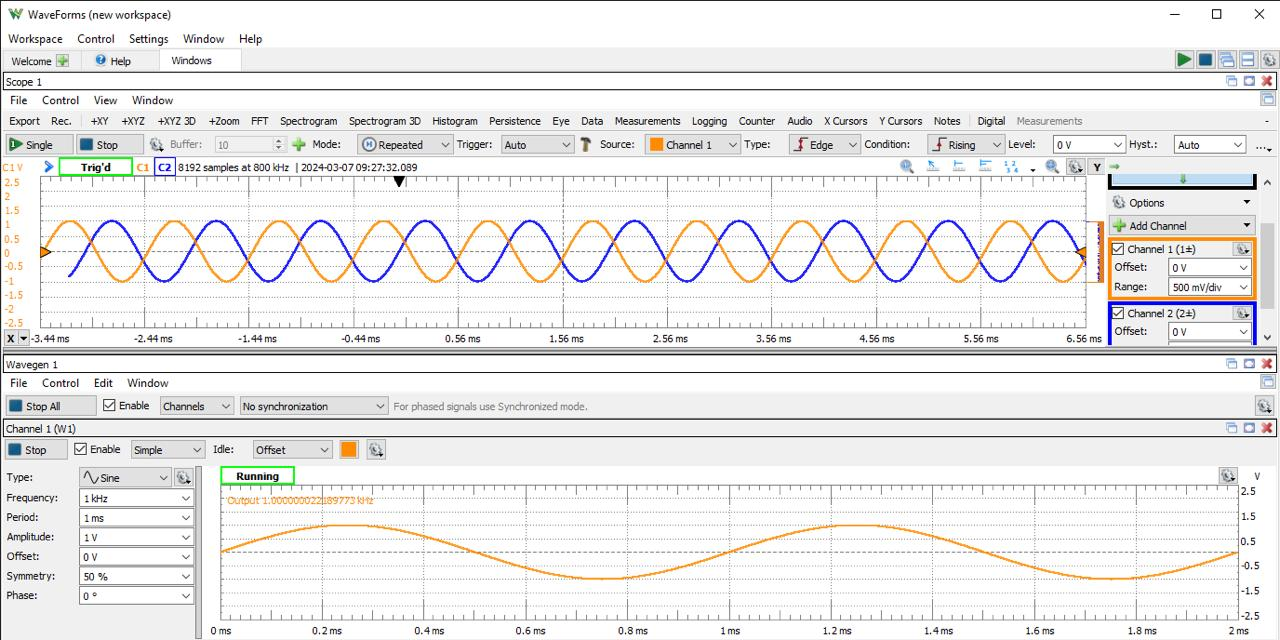
\includegraphics[width=0.99\textwidth]{unity_gain.jpg}
		\caption{The simulation plot with unity gain}
		\label{fig:unity}
	\end{figure}
	
	\begin{figure}[htbp]
		\centering
		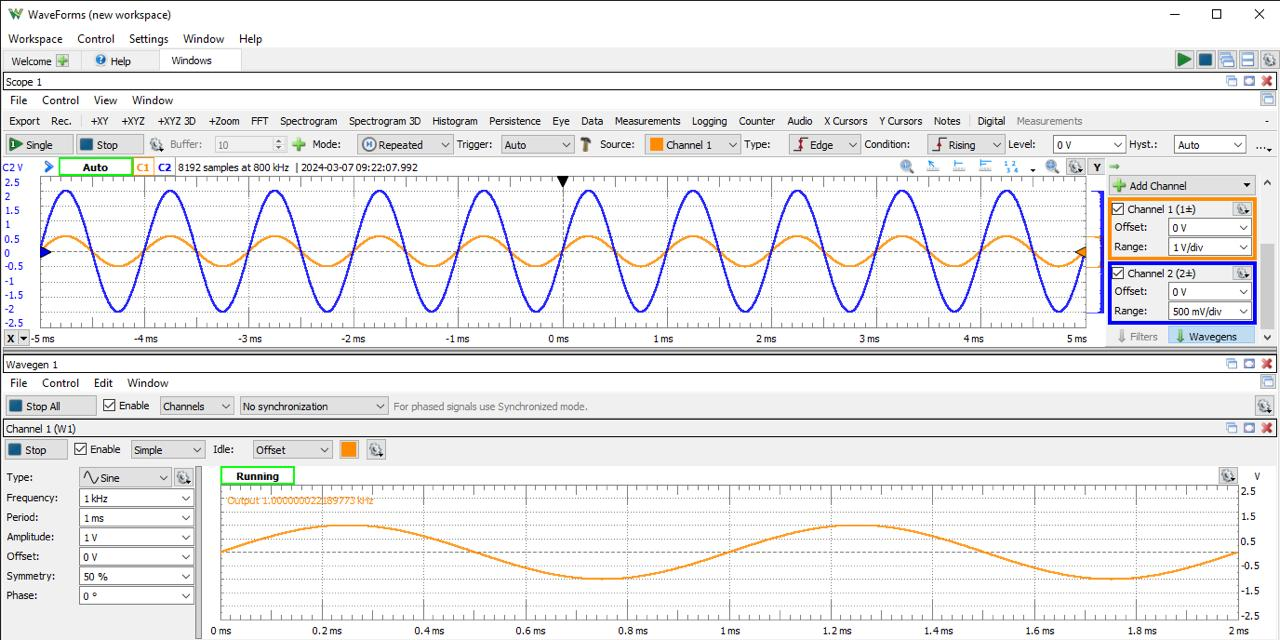
\includegraphics[width=0.99\textwidth]{gain_2.jpg}
		\caption{The simulation plot with gain of 2}
		\label{fig:gain2}
	\end{figure}
	
		\begin{figure}[htbp]
		\centering
		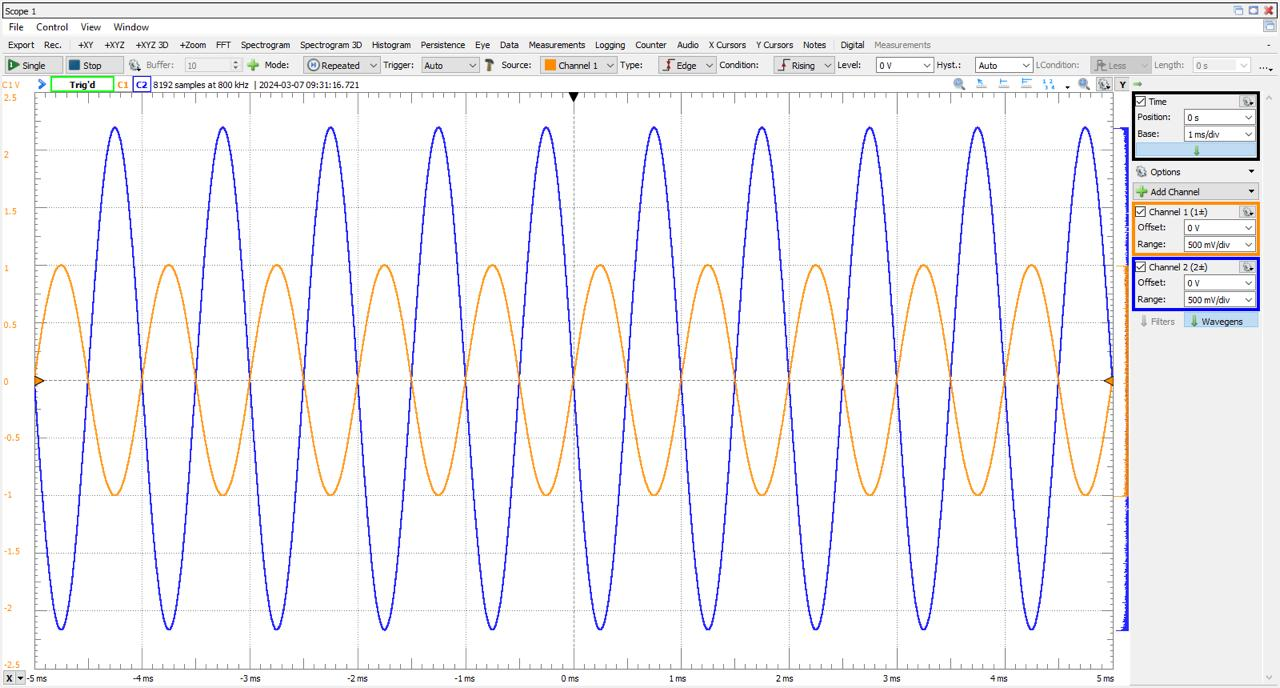
\includegraphics[width=0.99\textwidth]{gain2_4.jpg}
		\caption{The simulation plot with gain of 2.4}
		\label{fig:gain2_4}
	\end{figure}
	
	As shown in Figure \ref{fig:gain2}, the data points are densely concentrated in the lower left corner of the plot.
	
\end{document}
